% !TeX spellcheck = en_US
\section{Decline of HPV oncogenic HR infections in the long-term in Spain}\label{sec:onco_spain}
Here, we are going to repeat the study done in the previous section corresponding to HPV oncogenic HR 16/18/31/33/45/52/58, those GARDASIL9 protects. In this case, the study may give an idea about the future decline of the cases of HPV-related cancer, but taking into account that cancer use to appear after around $20$ years of persistent infection. 

As in the previous section, we are going to use the procedure explained in Section \ref{sec:decline}. The vaccination program started in Oct 2007.

The results can be seen in Figure \ref{fig:oncoESP}. For women, the herd immunity is present, in average, from $2010$ ($2$ years after the starting of the vaccination program). In the worst case, the herd immunity effect in women appears clearly after $39$ years, around $2047$.

In case of men, in average, the herd immunity appears from the very beginning ($0$ years, $2007.75$). As men are not vaccinated, the herd immunity can be visualized if the line is over zero. In the worst case, $2.5$ years ($2010.25$) are necessary to arise the threshold of the herd immunity. As in the previous cases, herd immunity effect does not appear for MSM.

We should note that, for HPV oncoviruses, the evolution of the decline is more uncertain than for HPV 6/11 after some years of vaccination campaign (see the confidence intervals). Then, if we want to predict when there will be a reduction of cases of cervical cancer after 2030, it may have a delay that could be of 15 years, in the worst case, although the average suggests very promising reductions.

\begin{figure}[!]
	\centering
	\begin{tabular}{cc}
		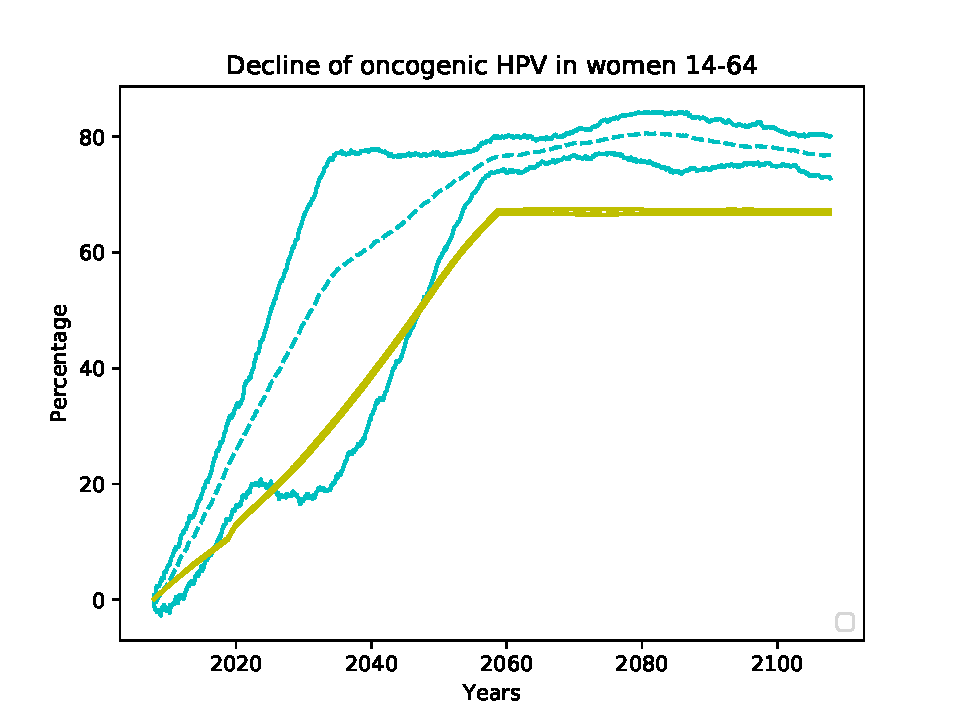
\includegraphics[width=0.5\linewidth]{IMGs/5.-Decline_onco/onco_muj.pdf}	& 
		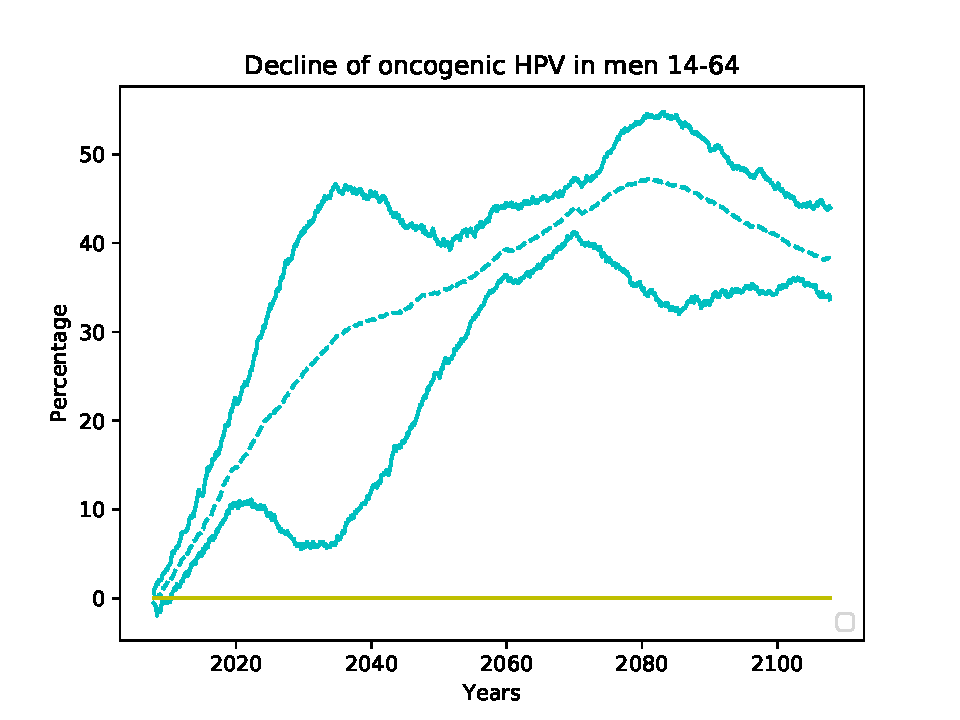
\includegraphics[width=0.5\linewidth]{IMGs/5.-Decline_onco/onco_hom.pdf}  \\ 
		(a)	& (b) \\ 
		\multicolumn{2}{c}{ 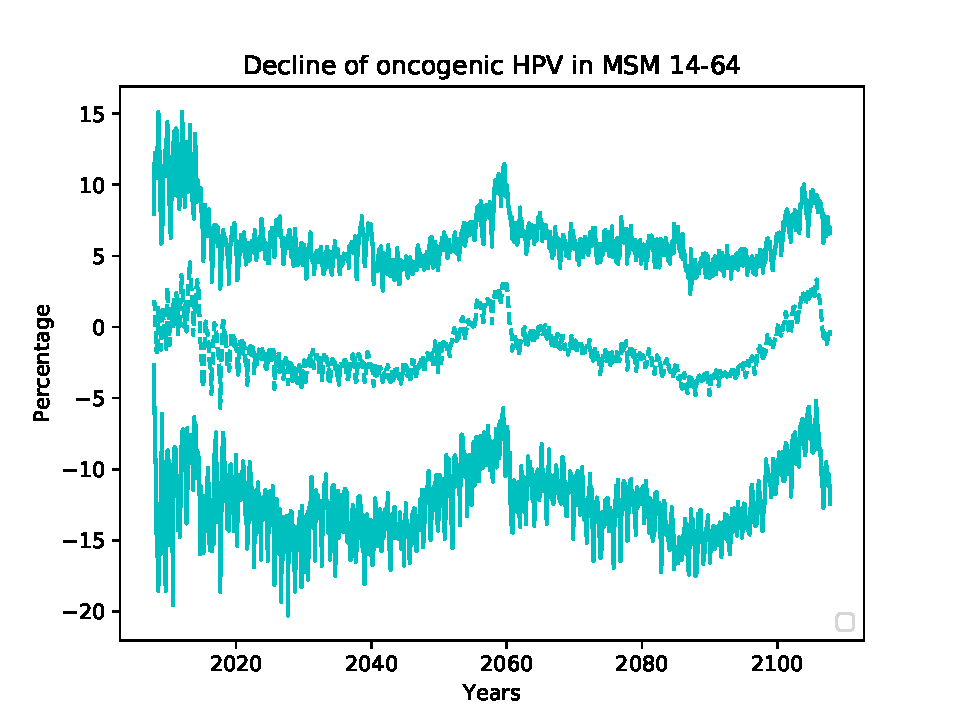
\includegraphics[width=0.5\linewidth]{IMGs/5.-Decline_onco/onco_MSM.pdf} } \\ 
		\multicolumn{2}{c}{(c)} \\ 
	\end{tabular} 
	\caption{Decline of HPV oncogenic HR infections in 14-64 years old women, men and MSM over the time, from Oct 2007, when the vaccination campaign started in Spain. In the women decline, we include the percentage of vaccinated women. It helps to visualize the herd immunity effect when the decline line is over the vaccination line. In case of men, the lines over the yellow abscissa line means effect of the herd immunity. For the MSM, there is not herd immunity effect.}
	\label{fig:oncoESP}
\end{figure}

In the Table \ref{tabla:oncoESP}, we can see when given percentages of decline of HPV oncogenic HR will be reached for women and men. As in the HPV LR case, it is not necessary a long time to achieve high percentages of decline for women and men in average. Furthermore, the decline percentages for oncogenic HPV types are worse than HPV LR 6/11.

\begin{table}[!h]
	\centering
	\begin{tabular}{c|ll}
		Decline & Women & Men \\ 
		\hline 
$ 30 \%$ & year 2022, CI95\% $[ 2019 , 2040 ]$ & year 2036, CI95\% $[ 2024 , 2054 ]$  \\
$ 40 \%$ & year 2027, CI95\% $[ 2023 , 2044 ]$ & year 2063, CI95\% $[ 2029 , 2065 ]$  \\
$ 50 \%$ & year 2031, CI95\% $[ 2025 , 2047 ]$ & year $-$, CI95\% $[ - , - ]$  \\
$ 60 \%$ & year 2039, CI95\% $[ 2028 , 2051 ]$ & year $-$, CI95\% $[ - , - ]$  \\
$ 70 \%$ & year 2050, CI95\% $[ 2032 , 2055 ]$ & year $-$, CI95\% $[ - , - ]$  \\
$ 80 \%$ & year 2076, CI95\% $[ 2058 , - ]$ & year $-$, CI95\% $[ - , - ]$  \\
    \end{tabular} 
	\caption{In this table we show when given percentages of oncogenic HPV decline in Spain with the current vaccination program will be reached over the time with a $95\%$ confidence interval. The symbol "$-$" means that this percentage is not reached in the simulation period. }
	\label{tabla:oncoESP}
\end{table}

